\documentclass{article}

% Language setting
% Replace `english' with e.g. `spanish' to change the document language
\usepackage[spanish]{babel}

\usepackage[letterpaper,top=2cm,bottom=5cm,left=3cm,right=3cm,marginparwidth=1.75cm]{geometry}

% Useful packages
\usepackage{amsmath}
\usepackage{graphicx}
\usepackage[colorlinks=true, allcolors=blue]{hyperref}
\usepackage{amssymb}
\usepackage{fancyhdr}
\usepackage{lipsum} % Para generar texto de ejemplo
\usepackage{multicol}
\usepackage{float}
\usepackage{booktabs}
\usepackage{tabularx}
\usepackage{array}
\pagestyle{fancy}

\fancyhf{} % Limpiar encabezado y pie de página por defecto
\setlength{\headheight}{70pt} % Ajuste del tamaño del encabezado (puedes aumentar este valor si es necesario)

% Definición del encabezado

\fancyhead[C]{%
    \begin{minipage}[c]{2.0cm}
        \centering
        \includegraphics[width=2.0cm]{imagenes/uta.png}
    \end{minipage}%
    \hfill
    \begin{minipage}[c]{8cm}
        \centering
        \small {\textbf{UNIVERSIDAD TÉCNICA DE AMBATO}} \\[0.1cm]
        \scriptsize \textit{FACULTAD DE INGENIERÍA EN SISTEMAS ELECTRÓNICA E INDUSTRIAL} \\[0.1cm]
        \scriptsize \textbf{CARRERA SOFTWARE - METODOLOGÍAS AGILES} \\[0.1cm]
        \scriptsize \textbf{CICLO ACADÉMICO: AGOSTO 2025 - ENERO 2026}
    \end{minipage}%
    \hfill
    \begin{minipage}[c]{2.0cm}
        \centering
        \includegraphics[width=2.0cm]{imagenes/fisei.png}
    \end{minipage}%
}

\begin{document}
\begin{center}
    {\large \textbf{INFORME DE TAREA}} \\
\end{center}

\section{Portada}
\begin{flushleft}
\begin{tabular}{ l p{9.5cm} }
    \textbf{Tema:} & Análisis, Arquitectura y Funcionamiento de la API REST del Sistema de Gestión de Citas para Clínica Médica Multiespecialidad (Clínica Ecuador) \\
    \textbf{Unidad de Organización Curricular:} & Profesional \\
    \textbf{Nivel y Paralelo:} & Nivel - Paralelo \\
    \textbf{Alumnos participantes:} & Apellidos y nombres (orden alfabético) \\
    & Apellidos y nombres (orden alfabético) \\
    & \dotfill \\
    \textbf{Asignatura:} & Arquitectura Orientada a Servicios (SOA) / Metodologías Ágiles \\
    \textbf{Docente:} & Ing. Nombre y Apellido, Mg. \\
\end{tabular}
\end{flushleft}


\section{Informe de la Tarea}
\subsection{Objetivos}
\subsubsection{General}
Analizar, documentar y demostrar el funcionamiento integral del \textbf{Sistema de Gestión de Citas para Clínica Médica Multiespecialidad (Clínica Ecuador)}, detallando su arquitectura orientada a servicios, los módulos que lo componen, la ubicación y consumo de su API REST con autenticación JWT y las evidencias visuales de su ejecución en todos los perfiles de usuario.

\subsubsection{Específicos}
\begin{itemize}
    \item Describir la estructura tecnológica del proyecto (\textit{backend} en Spring Boot 4.1.2 con Java 21, persistencia en MySQL y \textit{frontend} SPA en HTML5, CSS3 y JavaScript).
    \item Identificar cada uno de los \textit{endpoints} de la API REST, sus métodos HTTP, reglas de autorización por roles (\texttt{ROLE\_ADMIN}, \texttt{ROLE\_MEDICO}, \texttt{ROLE\_PACIENTE}) y el mecanismo de consumo desde el cliente web.
    \item Verificar y evidenciar mediante capturas de pantalla el comportamiento operativo de las vistas públicas, el registro e inicio de sesión, los portales de paciente, médico y administrador, así como las respuestas JSON directas de la API.
\end{itemize}


\subsection{Instrucciones}
Con base en el repositorio \texttt{ProyectoSOA} del Sistema de Gestión de Citas Médicas, se realizaron las siguientes actividades:
\begin{enumerate}
    \item Inspección del código fuente del \textit{backend} (controladores, servicios, repositorios, entidades, DTOs y configuración de seguridad) y del \textit{frontend} estático.
    \item Inicialización del esquema relacional \texttt{db\_clinica} en MySQL a partir del archivo \texttt{database/db\_clinica.sql} y carga de datos de prueba con contraseñas cifradas en BCrypt para los tres roles del sistema.
    \item Despliegue local del servicio Spring Boot en el puerto \texttt{8081} mediante Maven Wrapper (\texttt{mvnw}) y validación funcional en navegador web.
    \item Recopilación de evidencias gráficas de cada módulo funcional y de las respuestas directas de la API REST para su documentación técnica.
\end{enumerate}


\subsection{Listado de equipos, materiales y recursos}
\textbf{Listado de equipos y materiales generales empleados en la tarea:}
\begin{itemize}
    \item Computador personal con sistema operativo Windows 11.
    \item Java Development Kit (JDK 21) y Apache Maven Wrapper (\texttt{mvnw}).
    \item Framework Spring Boot 4.1.2 (Spring Web MVC, Spring Data JPA, Spring Security, Bean Validation) y librería JJWT 0.12.6.
    \item Servidor de base de datos relacional MySQL / MariaDB (XAMPP) con base de datos \texttt{db\_clinica}.
    \item Navegador web moderno con soporte para Fetch API, LocalStorage y visualización de respuestas JSON.
    \item Editor de código fuente y entorno de compilación \LaTeX{} para la elaboración del informe técnico.
\end{itemize}

\textbf{TAC (Tecnologías para el Aprendizaje y Conocimiento) empleados en la tarea:}
\begin{itemize}
    \item[$\square$] Plataformas educativas
    \item[$\boxtimes$] Simuladores y laboratorios virtuales
    \item[$\boxtimes$] Aplicaciones educativas
    \item[$\square$] Recursos audiovisuales
    \item[$\square$] Gamificación
    \item[$\boxtimes$] Inteligencia Artificial
    \item Otros (Especifique): \underline{Entorno local Spring Boot + MySQL + GitHub}
\end{itemize}


\subsection{Desarrollo de la Tarea (Actividades a Desarrollar)}

\subsubsection{¿Qué es el proyecto y qué componentes contiene?}
El proyecto \textbf{Clínica Ecuador (\texttt{clinica-medica})} es una aplicación web desarrollada bajo principios de \textbf{Arquitectura Orientada a Servicios (SOA)} y el estilo arquitectónico \textbf{REST} \cite{fielding2000}, orientada a la gestión integral de citas médicas en una clínica multiespecialidad. Su propósito es centralizar el catálogo de especialidades, el directorio de profesionales médicos, las fichas de pacientes y el ciclo de vida de las citas médicas (\texttt{PENDIENTE}, \texttt{CONFIRMADA}, \texttt{COMPLETADA} y \texttt{CANCELADA}), aplicando control de acceso basado en roles (\textit{RBAC}).

El sistema se organiza en una arquitectura por capas claramente desacopladas:
\begin{itemize}
    \item \textbf{Capa de Configuración y Seguridad (\texttt{com.clinicamedica.app.config}):} Contiene \texttt{SecurityConfig} (política \textit{stateless}, CORS, rutas públicas/protegidas y codificador BCrypt), \texttt{JwtUtils} (generación, firma HMAC-SHA y validación de tokens JWT), \texttt{JwtAuthorizationFilter} (filtro por petición que extrae el encabezado \texttt{Authorization: Bearer <token>}) y \texttt{GlobalExceptionHandler} (gestión centralizada de excepciones con respuestas JSON uniformes mediante \texttt{ResponseDto}).
    \item \textbf{Capa de Controladores REST (\texttt{com.clinicamedica.app.controller}):} Expone cinco servicios REST bajo el prefijo \texttt{/api}: \texttt{AuthController}, \texttt{EspecialidadController}, \texttt{MedicoController}, \texttt{PacienteController} y \texttt{CitaController}.
    \item \textbf{Capa de Servicios (\texttt{com.clinicamedica.app.service}):} Encapsula la lógica de negocio, validaciones de integridad (unicidad de cédula, correo y nombre de especialidad) y reglas de autorización según el usuario autenticado (\texttt{AuthService}, \texttt{CitaService}, \texttt{EspecialidadService}, \texttt{MedicoService} y \texttt{PacienteService}).
    \item \textbf{Capa de Persistencia (\texttt{entity} y \texttt{repository}):} Mapea mediante Spring Data JPA \cite{springboot2025} las siete tablas relacionales definidas en \texttt{database/db\_clinica.sql} sobre MySQL \cite{mysql2025}: \texttt{usuarios}, \texttt{roles}, \texttt{usuario\_roles}, \texttt{especialidades}, \texttt{pacientes}, \texttt{medicos} y \texttt{citas}.
    \item \textbf{Capa de Transferencia de Datos (\texttt{dto}):} Define contratos JSON seguros (\texttt{LoginDto}, \texttt{RegistroDto}, \texttt{MedicoDto}, \texttt{CitaDto} y \texttt{ResponseDto}) que evitan exponer directamente entidades sensibles como contraseñas cifradas.
    \item \textbf{Capa de Presentación SPA (\texttt{src/main/resources/static}):} Interfaz web responsiva de una sola página (\texttt{index.html}, \texttt{css/styles.css}) servida desde el mismo puerto \texttt{8081}, apoyada por tres módulos JavaScript: \texttt{auth.js} (gestión de sesión, cliente HTTP y navegación dinámica por rol), \texttt{citas.js} (consumo de la API para todas las vistas y formularios CRUD) y \texttt{ui.js} (modales accesibles, menú móvil y formulario de contacto).
\end{itemize}

\subsubsection{¿Dónde se ocupa la API REST y cuáles son sus endpoints?}
Toda la comunicación entre la interfaz web y el servidor ocurre a través de la API REST alojada en \texttt{http://localhost:8081/api/*}. No existe renderizado de vistas en el servidor; las páginas dinámicas del sitio público y de los tres portales de usuario obtienen y modifican datos exclusivamente mediante peticiones HTTP JSON. La Tabla~\ref{tab:endpoints} resume el catálogo completo de \textit{endpoints} expuestos por el \textit{backend}.

\begin{table}[H]
\centering
\caption{Catálogo de endpoints de la API REST de Clínica Ecuador.}
\label{tab:endpoints}
\scriptsize
\begin{tabularx}{\textwidth}{@{} l l l X @{}}
\toprule
\textbf{Controlador} & \textbf{Método} & \textbf{Endpoint} & \textbf{Acceso y Función} \\
\midrule
\texttt{AuthController} & POST & \texttt{/api/auth/login} & Público. Autentica credenciales y emite token JWT + rol. \\
& POST & \texttt{/api/auth/registro} & Público (alias \texttt{/register}). Registra usuario y ficha de paciente con \texttt{ROLE\_PACIENTE}. \\
& GET & \texttt{/api/auth/perfil} & Autenticado. Devuelve datos básicos y roles del usuario en sesión. \\
\midrule
\texttt{Especialidad-} & GET & \texttt{/api/especialidades} & Público. Lista todas las especialidades médicas disponibles. \\
\texttt{Controller} & GET & \texttt{/api/especialidades/\{id\}} & Público. Obtiene el detalle de una especialidad por ID. \\
& POST & \texttt{/api/especialidades} & \texttt{ROLE\_ADMIN}. Crea una nueva especialidad médica. \\
& PUT & \texttt{/api/especialidades/\{id\}} & \texttt{ROLE\_ADMIN}. Actualiza nombre y descripción. \\
& DELETE & \texttt{/api/especialidades/\{id\}} & \texttt{ROLE\_ADMIN}. Elimina una especialidad del catálogo. \\
\midrule
\texttt{Medico-} & GET & \texttt{/api/medicos} & Público. Lista médicos; admite filtro \texttt{?especialidadId=}. \\
\texttt{Controller} & GET & \texttt{/api/medicos/\{id\}} & Público. Obtiene ficha DTO de un médico específico. \\
& GET & \texttt{/api/medicos/mi-perfil} & \texttt{ROLE\_MEDICO}. Retorna el perfil profesional del médico autenticado. \\
& GET & \texttt{/api/medicos/mis-pacientes} & \texttt{ROLE\_MEDICO}. Lista pacientes distintos atendidos por el médico. \\
& POST & \texttt{/api/medicos} & \texttt{ROLE\_ADMIN}. Crea cuenta \texttt{ROLE\_MEDICO} (BCrypt) y ficha médica. \\
& PUT & \texttt{/api/medicos/\{id\}} & \texttt{ROLE\_ADMIN}. Actualiza datos del médico y contraseña opcional. \\
& DELETE & \texttt{/api/medicos/\{id\}} & \texttt{ROLE\_ADMIN}. Elimina al médico y su usuario vinculado. \\
\midrule
\texttt{Paciente-} & GET & \texttt{/api/pacientes} & \texttt{ROLE\_ADMIN}, \texttt{ROLE\_MEDICO}. Lista el directorio de pacientes. \\
\texttt{Controller} & GET & \texttt{/api/pacientes/\{id\}} & \texttt{ROLE\_ADMIN}, \texttt{ROLE\_MEDICO}. Consulta un paciente por ID. \\
& GET & \texttt{/api/pacientes/mi-perfil} & \texttt{ROLE\_PACIENTE}. Devuelve la ficha personal del paciente en sesión. \\
& POST & \texttt{/api/pacientes} & \texttt{ROLE\_ADMIN}. Registra una ficha de paciente. \\
& PUT & \texttt{/api/pacientes/\{id\}} & \texttt{ROLE\_ADMIN}. Actualiza los datos de un paciente. \\
& DELETE & \texttt{/api/pacientes/\{id\}} & \texttt{ROLE\_ADMIN}. Elimina un registro de paciente. \\
\midrule
\texttt{CitaController} & GET & \texttt{/api/citas} & Autenticado. Filtra según rol (\texttt{fecha}, \texttt{estado}, \texttt{medicoId}, \texttt{pacienteId}). \\
& GET & \texttt{/api/citas/\{id\}} & Autenticado. Verifica pertenencia de la cita antes de responder. \\
& POST & \texttt{/api/citas} & Autenticado. Agenda una nueva cita con estado inicial \texttt{PENDIENTE}. \\
& PUT & \texttt{/api/citas/\{id\}} & Autenticado. Reasignación completa por \texttt{ADMIN} o cambio de estado. \\
& PATCH & \texttt{/api/citas/\{id\}/estado} & Autenticado. Cambia estado (Paciente: solo cancela pendientes; Médico: confirma, completa o cancela). \\
& DELETE & \texttt{/api/citas/\{id\}} & \texttt{ROLE\_ADMIN}. Elimina permanentemente una cita médica. \\
\bottomrule
\end{tabularx}
\end{table}

\subsubsection{¿Cómo funciona el consumo de la API y la seguridad JWT?}
El funcionamiento operativo del sistema sigue un flujo \textit{stateless} (sin sesiones en servidor) basado en JSON Web Tokens (JWT) \cite{rfc7519}:

\begin{enumerate}
    \item \textbf{Autenticación y emisión de token:} Cuando un usuario envía sus credenciales en el formulario de inicio de sesión, \texttt{auth.js} ejecuta \texttt{Auth.login()}, que realiza un \texttt{POST /api/auth/login}. En el servidor, \texttt{AuthService} valida el correo y la contraseña cifrada con BCrypt mediante \texttt{AuthenticationManager}, genera un token firmado con HMAC-SHA (\texttt{JwtUtils.generateToken()}) con expiración de 24 horas (\texttt{86400000 ms}) y devuelve un objeto \texttt{ResponseDto} con \texttt{token}, \texttt{rol} y \texttt{datos}.
    \item \textbf{Almacenamiento en el cliente y cliente HTTP centralizado:} El cliente guarda \texttt{jwt\_token}, \texttt{user\_rol}, \texttt{user\_email} y \texttt{user\_datos} en \texttt{localStorage}. Todas las llamadas posteriores pasan por el método centralizado \texttt{Auth.request(endpoint, options)} en \texttt{auth.js}, el cual utiliza la \textit{Fetch API} \cite{mdnfetch}, establece \texttt{Content-Type: application/json} e inyecta automáticamente la cabecera \texttt{Authorization: Bearer <token>} cuando existe una sesión activa.
    \item \textbf{Validación en el servidor por cada petición:} Antes de llegar a cualquier controlador, \texttt{JwtAuthorizationFilter} intercepta la solicitud, extrae el token del encabezado \texttt{Authorization}, verifica la firma y fecha de expiración con \texttt{JwtUtils.isTokenValid()}, carga los permisos del usuario y establece el contexto en \texttt{SecurityContextHolder}. Si el token falta o expiró en una ruta protegida, \texttt{SecurityConfig} responde HTTP \texttt{401 Unauthorized}, lo que provoca que \texttt{Auth.request()} limpie la sesión local y redirija automáticamente al inicio de sesión.
    \item \textbf{Consumo diferenciado por vista y rol en \texttt{citas.js}:}
    \begin{itemize}
        \item \textit{Vistas públicas:} \texttt{cargarEspecialidadesPublicas()} consume \texttt{GET /api/especialidades} y \texttt{cargarMedicosPublicos()} consume \texttt{GET /api/medicos} sin requerir autenticación.
        \item \textit{Flujo del Paciente:} Al abrir ``Agendar nueva cita'', \texttt{prepararAgendamiento()} llena el selector de especialidades y, al cambiar la selección, invoca dinámicamente \texttt{GET /api/medicos?especialidadId=\{id\}} para mostrar solo los especialistas correspondientes. Al confirmar, envía \texttt{POST /api/citas}. En ``Mis citas médicas'' consume \texttt{GET /api/citas} (el servidor filtra automáticamente por el paciente autenticado) y permite cancelar citas pendientes mediante \texttt{PATCH /api/citas/\{id\}/estado}.
        \item \textit{Flujo del Médico:} Consume \texttt{GET /api/citas?fecha=...\&estado=...} para su agenda personal, cambia estados a \texttt{CONFIRMADA}, \texttt{COMPLETADA} o \texttt{CANCELADA} vía \texttt{PATCH}, consulta su historial de pacientes en \texttt{GET /api/medicos/mis-pacientes} y su ficha en \texttt{GET /api/medicos/mi-perfil}.
        \item \textit{Flujo del Administrador:} Supervisa todas las citas del sistema con filtros globales, reasigna médicos o estados vía \texttt{PUT /api/citas/\{id\}}, elimina citas con \texttt{DELETE /api/citas/\{id\}}, y ejecuta operaciones CRUD completas sobre médicos (\texttt{/api/medicos}), especialidades (\texttt{/api/especialidades}) y consulta el directorio de pacientes (\texttt{GET /api/pacientes}).
    \end{itemize}
\end{enumerate}


\subsection{Resultados obtenidos}
Tras inicializar la base de datos \texttt{db\_clinica} y ejecutar el servidor Spring Boot en \texttt{http://localhost:8081}, se verificó el funcionamiento correcto de todos los módulos y \textit{endpoints}. A continuación se presentan las evidencias capturadas durante la ejecución real del sistema.

\subsubsection{Portal Público y Consumo de Catálogos}
La Figura~\ref{fig:inicio} muestra la página de inicio de Clínica Ecuador con la barra de navegación pública, indicadores institucionales y accesos directos a registro e inicio de sesión. Las Figuras~\ref{fig:esp_pub} y~\ref{fig:med_pub} evidencian la carga dinámica de especialidades y personal médico directamente desde \texttt{GET /api/especialidades} y \texttt{GET /api/medicos}.

\begin{figure}[H]
    \centering
    
\includegraphics[width=0.88\textwidth]{imagenes/01_inicio.png}
    \caption{Vista principal (Inicio) de Clínica Ecuador servida en \texttt{http://localhost:8081}.}
    \label{fig:inicio}
\end{figure}

\begin{figure}[H]
    \centering
    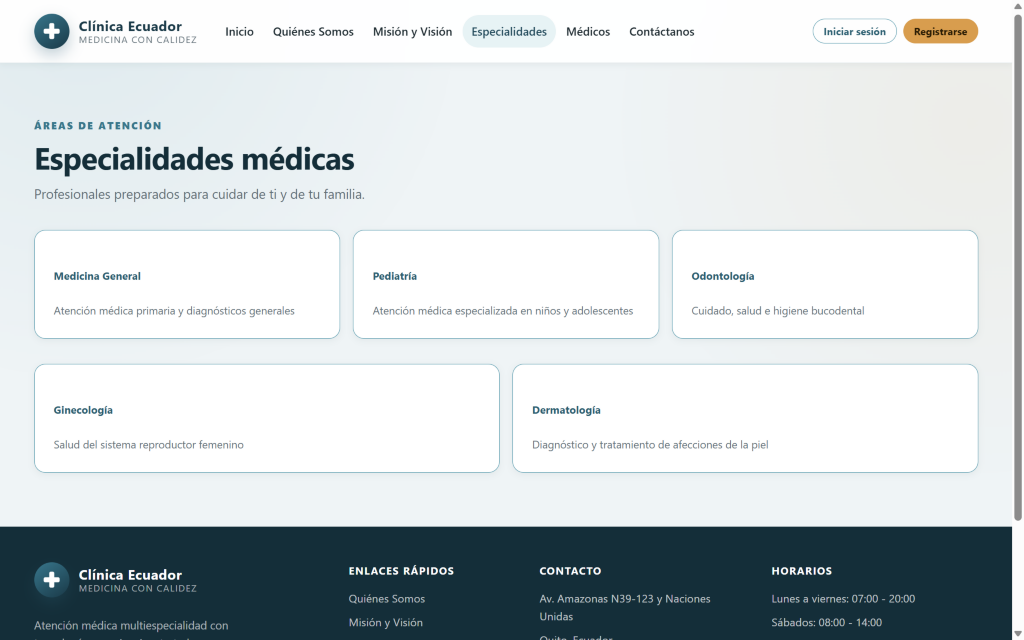
\includegraphics[width=0.88\textwidth]{imagenes/02_especialidades_publicas.png}
    \caption{Catálogo público de especialidades médicas cargado desde \texttt{GET /api/especialidades}.}
    \label{fig:esp_pub}
\end{figure}

\begin{figure}[H]
    \centering
    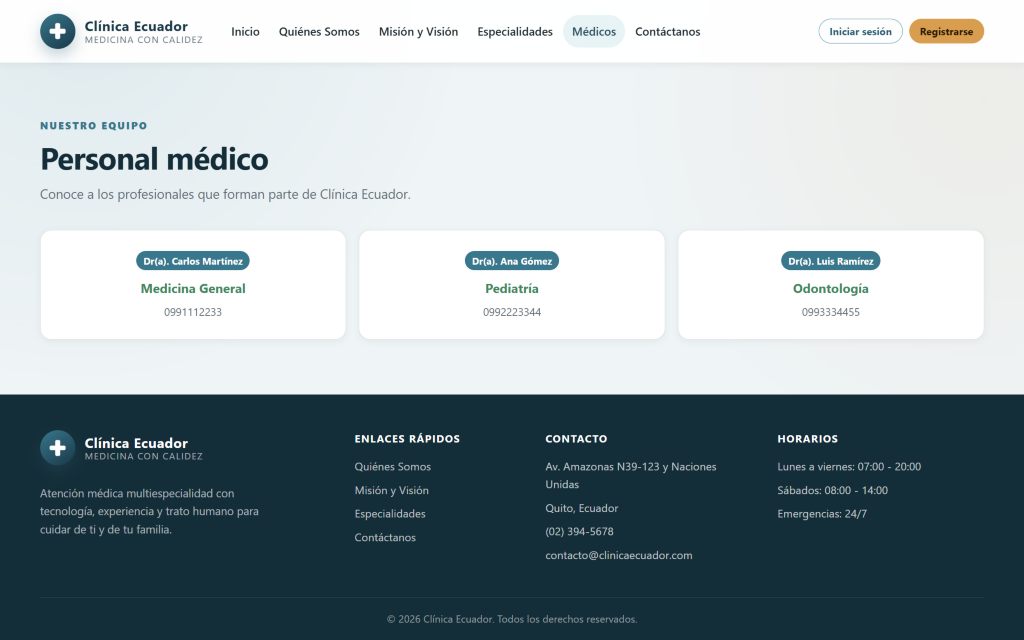
\includegraphics[width=0.88\textwidth]{imagenes/03_medicos_publicos.png}
    \caption{Directorio público de personal médico cargado desde \texttt{GET /api/medicos}.}
    \label{fig:med_pub}
\end{figure}

\subsubsection{Registro de Pacientes e Inicio de Sesión (JWT)}
En la Figura~\ref{fig:registro} se presenta el formulario de registro de nuevos pacientes, el cual consume \texttt{POST /api/auth/registro} validando cédula única, correo y contraseña mínima de 6 caracteres. La Figura~\ref{fig:login} muestra la vista de autenticación que invoca \texttt{POST /api/auth/login} para obtener el token JWT y redirigir según el rol.

\begin{figure}[H]
    \centering
    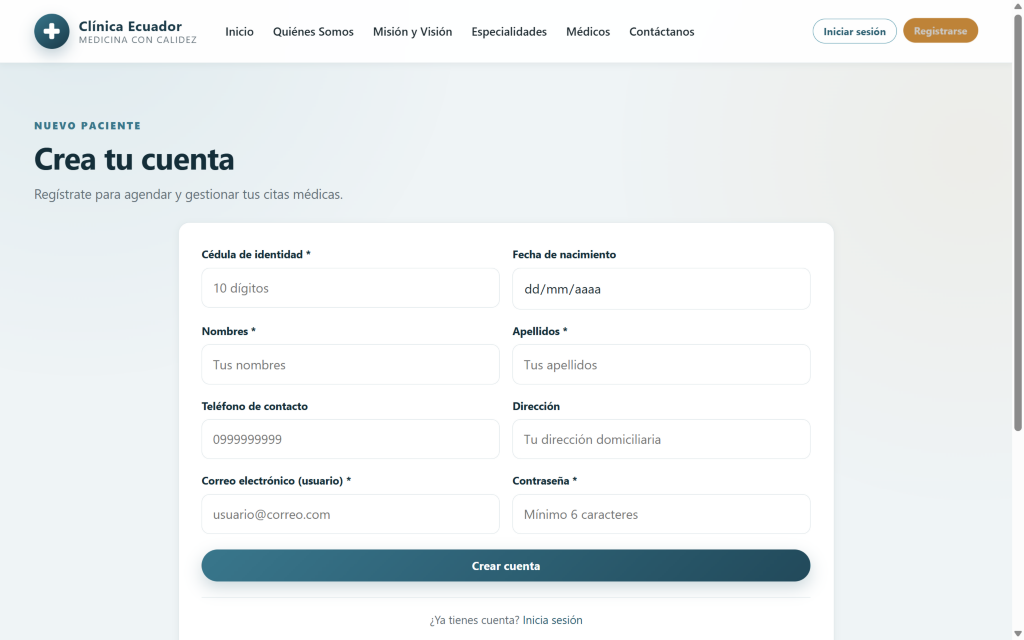
\includegraphics[width=0.88\textwidth]{imagenes/04_registro_paciente.png}
    \caption{Formulario de registro de nuevos pacientes (\texttt{POST /api/auth/registro}).}
    \label{fig:registro}
\end{figure}

\begin{figure}[H]
    \centering
    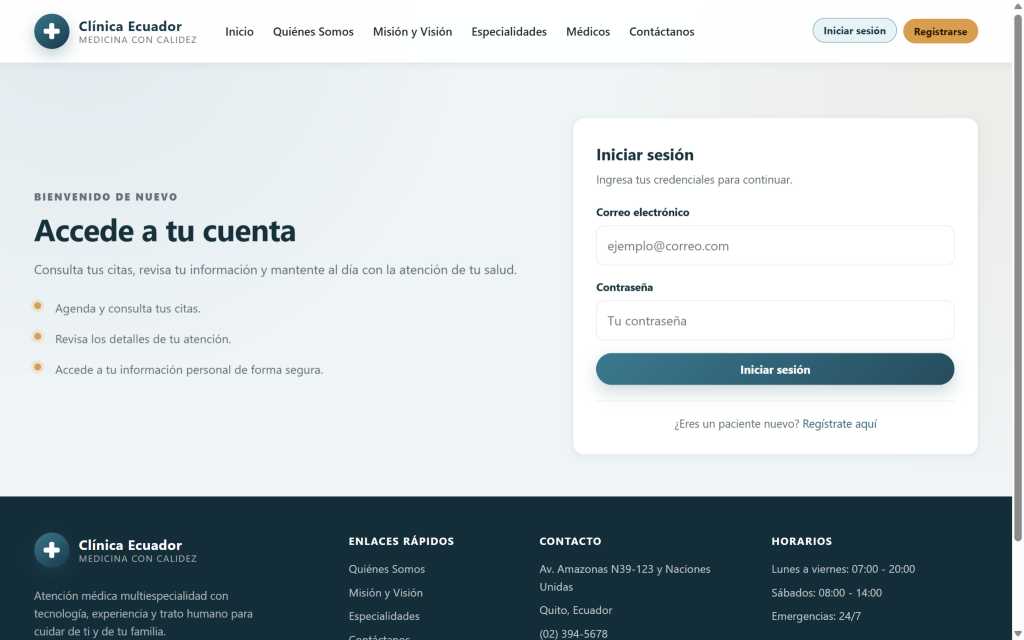
\includegraphics[width=0.88\textwidth]{imagenes/05_login.png}
    \caption{Interfaz de inicio de sesión para autenticación JWT (\texttt{POST /api/auth/login}).}
    \label{fig:login}
\end{figure}

\subsubsection{Portal del Paciente (\texttt{ROLE\_PACIENTE})}
Al autenticarse como paciente (\texttt{paciente@clinicaecuador.com}), la interfaz adapta la barra de navegación y muestra sus citas médicas (Figura~\ref{fig:pac_citas}), permitiendo cancelar únicamente aquellas en estado \texttt{PENDIENTE}. La Figura~\ref{fig:pac_agendar} demuestra la carga en cascada de médicos al seleccionar una especialidad (\texttt{GET /api/medicos?especialidadId=1}) para agendar una nueva consulta, y la Figura~\ref{fig:pac_perfil} muestra la ficha personal obtenida desde \texttt{GET /api/pacientes/mi-perfil}.

\begin{figure}[H]
    \centering
    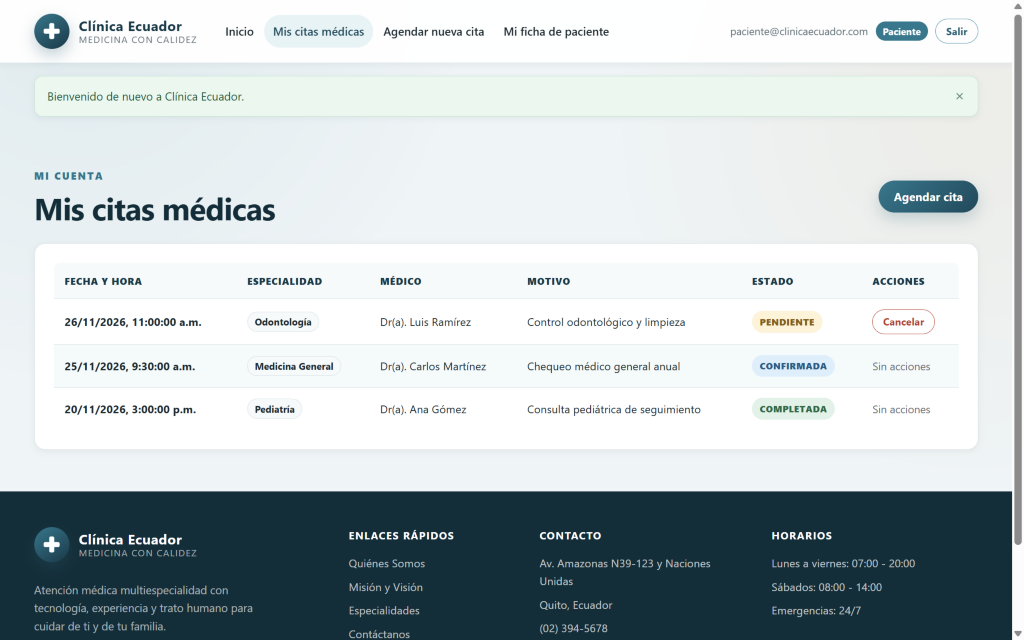
\includegraphics[width=0.88\textwidth]{imagenes/06_paciente_citas.png}
    \caption{Portal Paciente: listado de citas médicas propias (\texttt{GET /api/citas}) y botón de cancelación.}
    \label{fig:pac_citas}
\end{figure}

\begin{figure}[H]
    \centering
    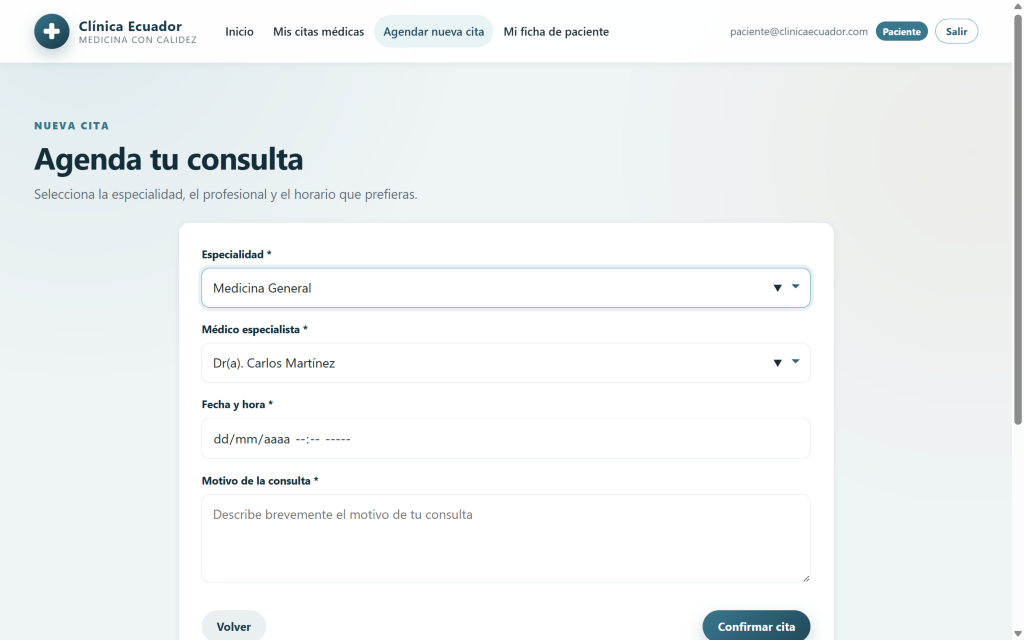
\includegraphics[width=0.88\textwidth]{imagenes/07_paciente_agendar.png}
    \caption{Portal Paciente: agendamiento con filtro dinámico de médicos por especialidad (\texttt{POST /api/citas}).}
    \label{fig:pac_agendar}
\end{figure}

\begin{figure}[H]
    \centering
    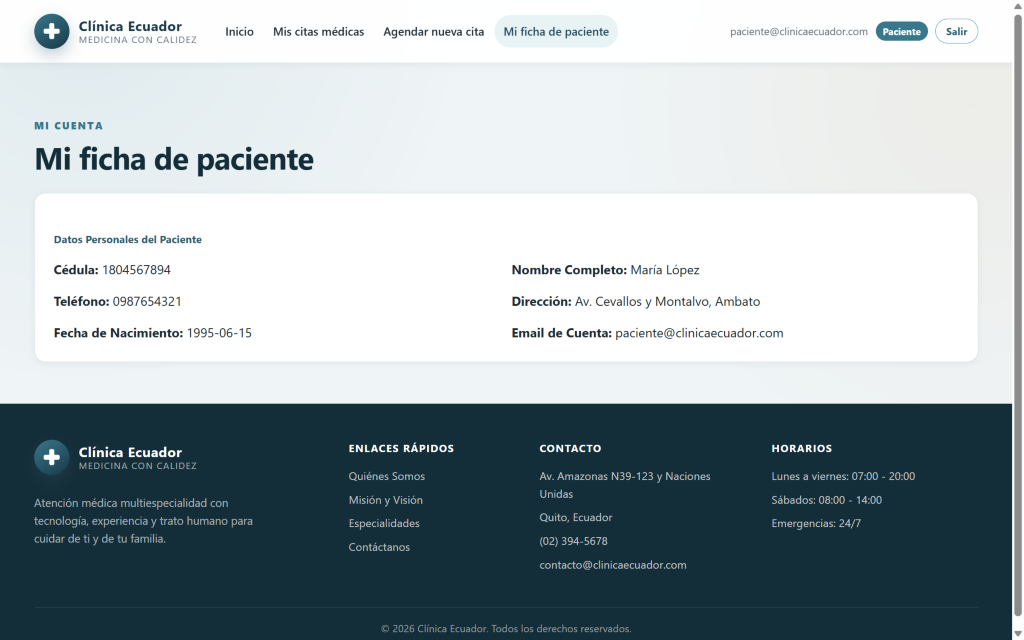
\includegraphics[width=0.88\textwidth]{imagenes/08_paciente_perfil.png}
    \caption{Portal Paciente: ficha de datos personales consultada en \texttt{GET /api/pacientes/mi-perfil}.}
    \label{fig:pac_perfil}
\end{figure}

\subsubsection{Portal del Médico (\texttt{ROLE\_MEDICO})}
Al ingresar con una cuenta médica (\texttt{dr.martinez@clinicaecuador.com}), el sistema habilita la gestión de agenda con filtros por fecha y estado y controles para confirmar, completar o cancelar citas vía \texttt{PATCH /api/citas/\{id\}/estado} (Figura~\ref{fig:med_agenda}). Asimismo, el profesional accede al historial de pacientes atendidos desde \texttt{GET /api/medicos/mis-pacientes} (Figura~\ref{fig:med_pac}) y a su ficha profesional desde \texttt{GET /api/medicos/mi-perfil} (Figura~\ref{fig:med_perfil}).

\begin{figure}[H]
    \centering
    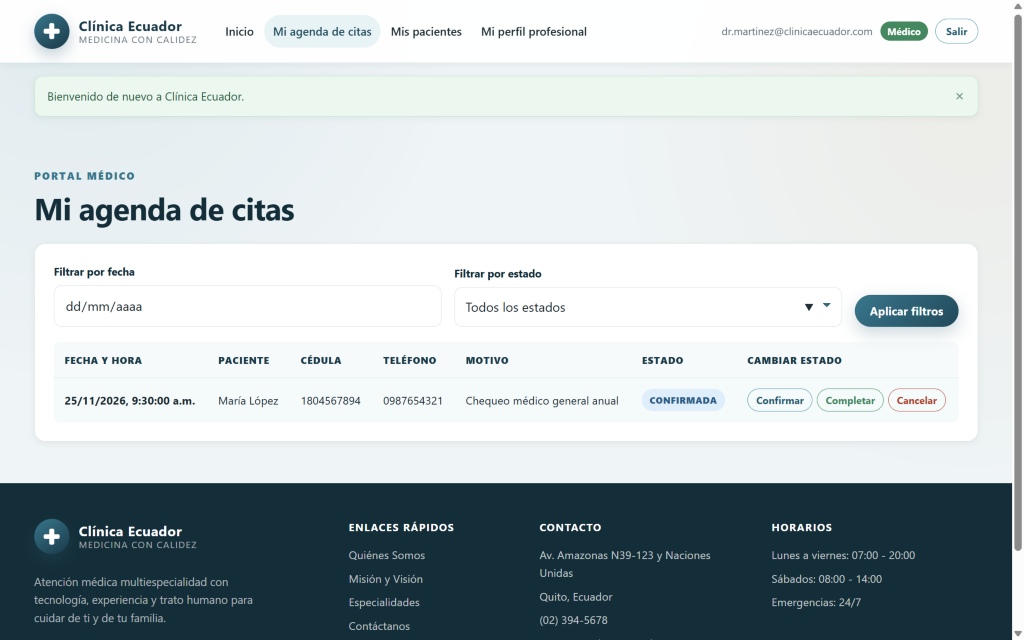
\includegraphics[width=0.88\textwidth]{imagenes/09_medico_agenda.png}
    \caption{Portal Médico: agenda de citas con filtros y acciones de cambio de estado.}
    \label{fig:med_agenda}
\end{figure}

\begin{figure}[H]
    \centering
    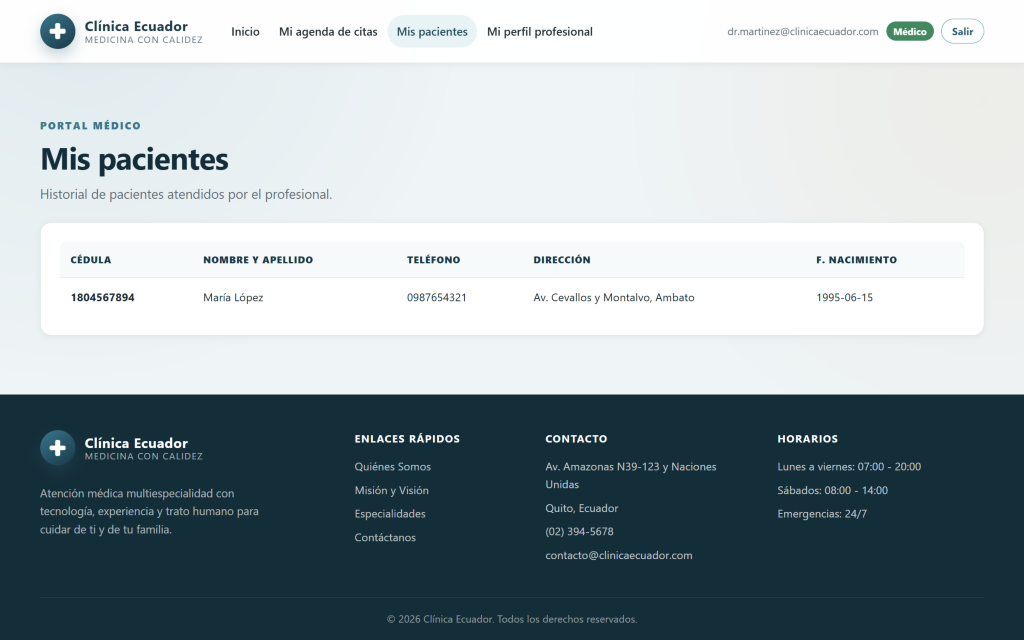
\includegraphics[width=0.88\textwidth]{imagenes/10_medico_pacientes.png}
    \caption{Portal Médico: listado de pacientes atendidos (\texttt{GET /api/medicos/mis-pacientes}).}
    \label{fig:med_pac}
\end{figure}

\begin{figure}[H]
    \centering
    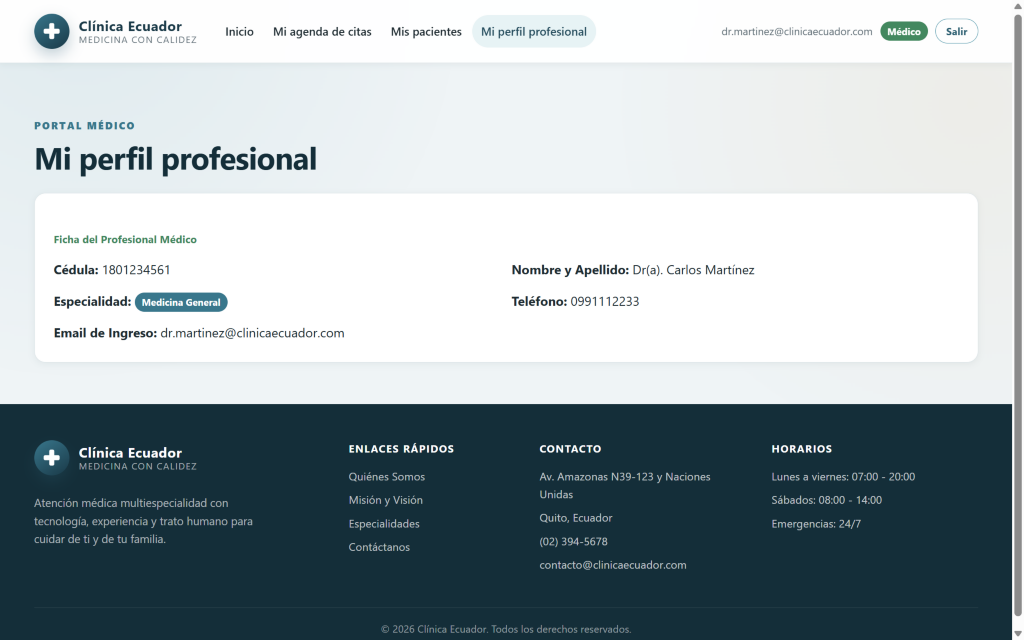
\includegraphics[width=0.88\textwidth]{imagenes/11_medico_perfil.png}
    \caption{Portal Médico: ficha profesional del especialista (\texttt{GET /api/medicos/mi-perfil}).}
    \label{fig:med_perfil}
\end{figure}

\subsubsection{Panel del Administrador (\texttt{ROLE\_ADMIN})}
Con el rol administrador (\texttt{admin@clinicaecuador.com}) se desbloquea el control global de la clínica: supervisión, reasignación y eliminación de citas (Figura~\ref{fig:adm_citas}), gestión CRUD de médicos y sus cuentas de acceso (Figura~\ref{fig:adm_med}), administración del catálogo de especialidades (Figura~\ref{fig:adm_esp}) y consulta del directorio completo de pacientes registrados (Figura~\ref{fig:adm_pac}).

\begin{figure}[H]
    \centering
    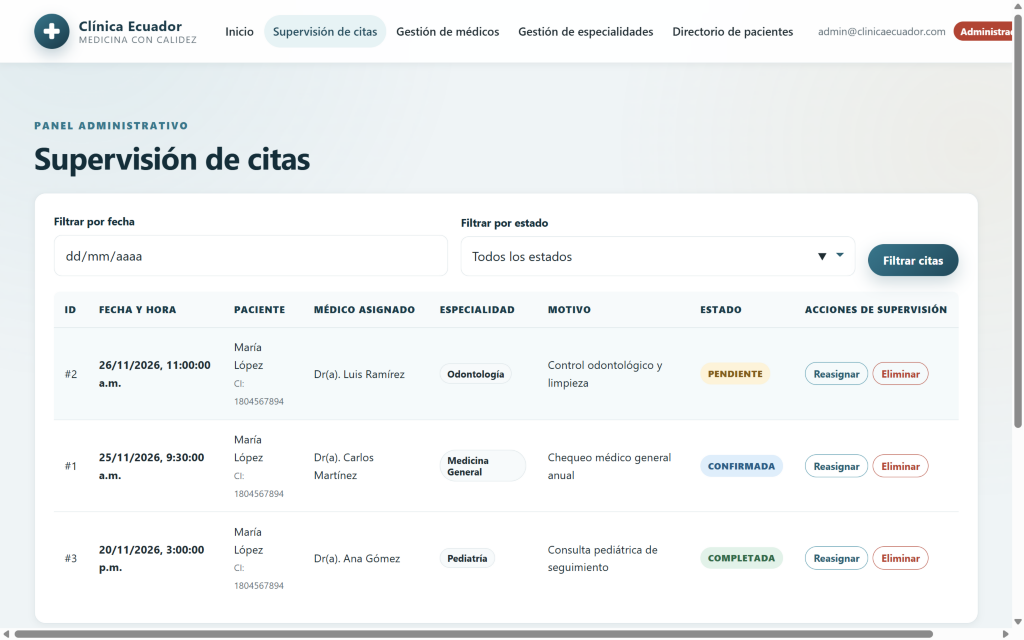
\includegraphics[width=0.88\textwidth]{imagenes/12_admin_citas.png}
    \caption{Panel Administrador: supervisión global de citas con opciones de reasignación y eliminación.}
    \label{fig:adm_citas}
\end{figure}

\begin{figure}[H]
    \centering
    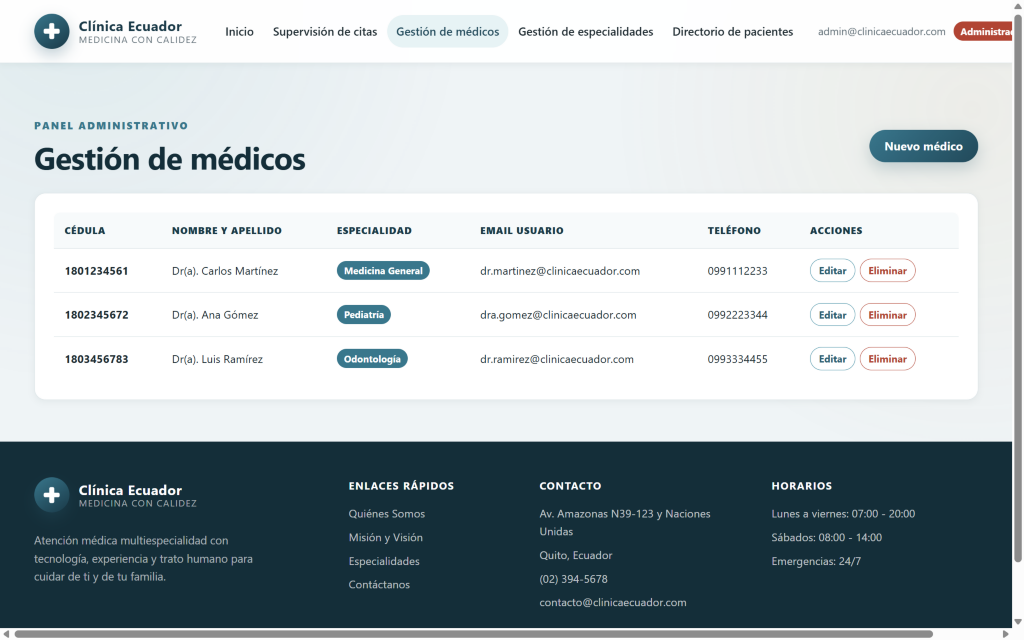
\includegraphics[width=0.88\textwidth]{imagenes/13_admin_medicos.png}
    \caption{Panel Administrador: gestión CRUD de médicos (\texttt{/api/medicos}).}
    \label{fig:adm_med}
\end{figure}

\begin{figure}[H]
    \centering
    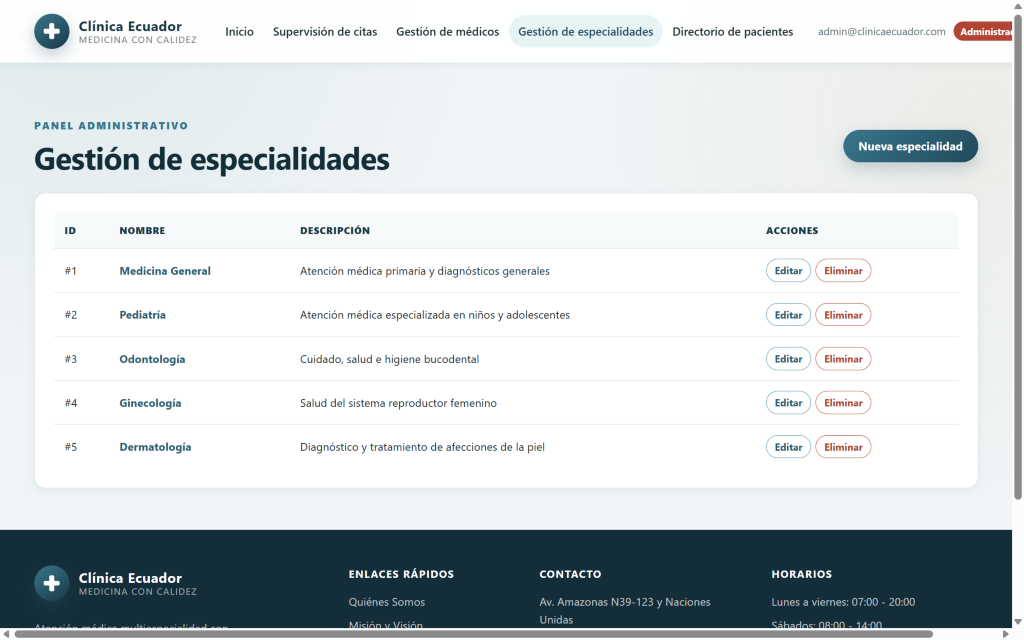
\includegraphics[width=0.88\textwidth]{imagenes/14_admin_especialidades.png}
    \caption{Panel Administrador: gestión CRUD de especialidades médicas (\texttt{/api/especialidades}).}
    \label{fig:adm_esp}
\end{figure}

\begin{figure}[H]
    \centering
    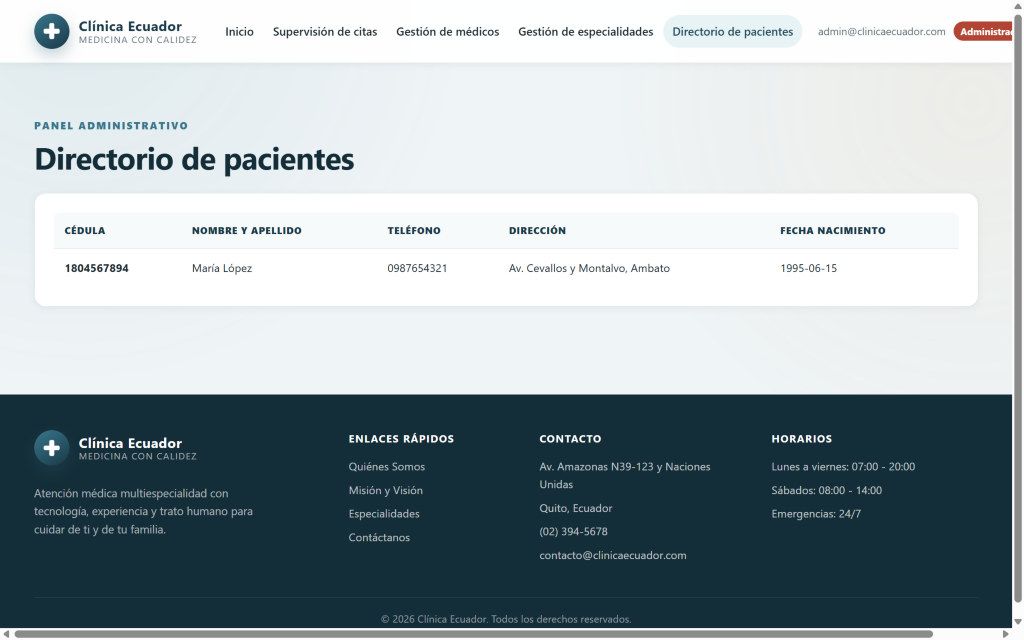
\includegraphics[width=0.88\textwidth]{imagenes/15_admin_pacientes.png}
    \caption{Panel Administrador: directorio general de pacientes (\texttt{GET /api/pacientes}).}
    \label{fig:adm_pac}
\end{figure}

\subsubsection{Verificación Directa de Respuestas JSON de la API REST}
Finalmente, las Figuras~\ref{fig:api_esp} y~\ref{fig:api_med} confirman las respuestas JSON estructuradas que devuelve el servidor Spring Boot al consultar directamente los \textit{endpoints} públicos \texttt{/api/especialidades} y \texttt{/api/medicos}, validando el cumplimiento de los contratos DTO y la codificación UTF-8.

\begin{figure}[H]
    \centering
    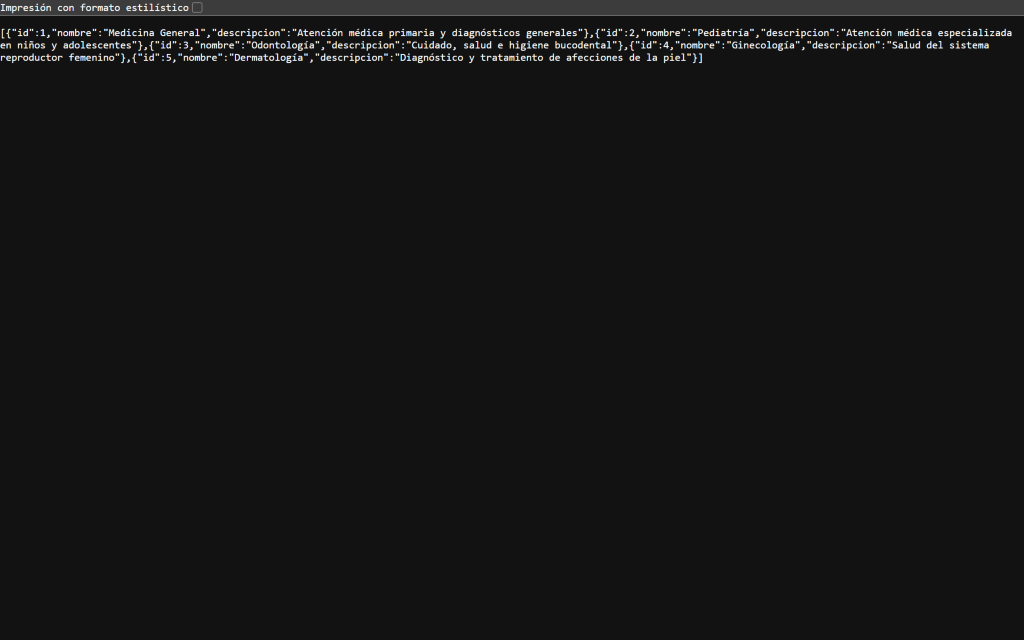
\includegraphics[width=0.88\textwidth]{imagenes/16_api_especialidades.png}
    \caption{Respuesta JSON directa del endpoint \texttt{GET http://localhost:8081/api/especialidades}.}
    \label{fig:api_esp}
\end{figure}

\begin{figure}[H]
    \centering
    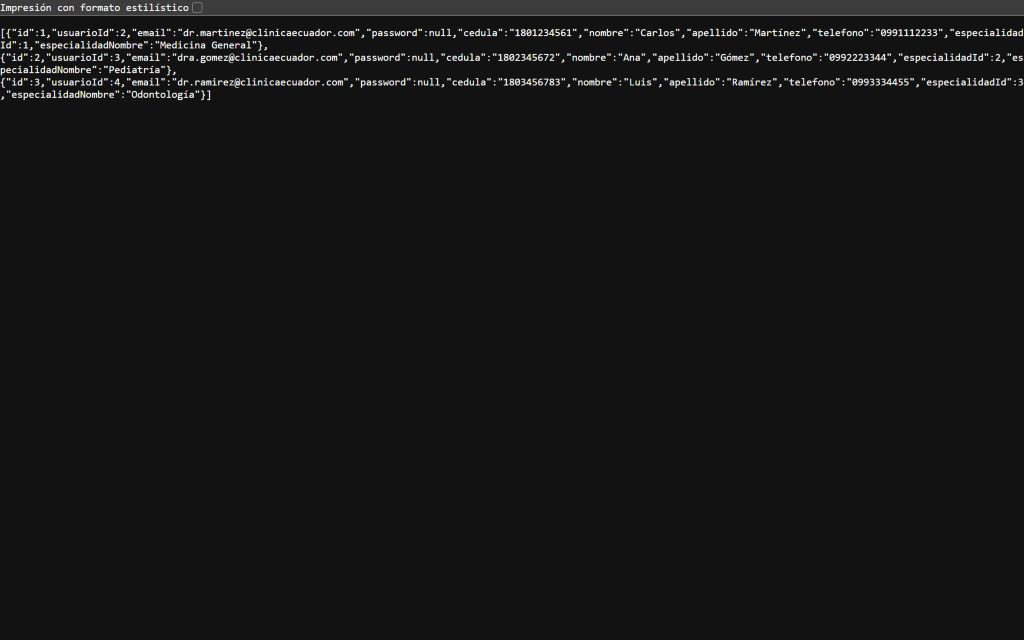
\includegraphics[width=0.88\textwidth]{imagenes/17_api_medicos.png}
    \caption{Respuesta JSON directa del endpoint \texttt{GET http://localhost:8081/api/medicos}.}
    \label{fig:api_med}
\end{figure}


%Especifique las TAC's utilizadas en la Tarea.
\subsection{Habilidades blandas empleadas en la tarea}
\begin{itemize}
    \item[$\square$] Liderazgo
    \item[$\boxtimes$] Trabajo en equipo
    \item[$\boxtimes$] Comunicación asertiva
    \item[$\square$] La empatía
    \item[$\boxtimes$] Pensamiento crítico
    \item[$\square$] Flexibilidad
    \item[$\square$] La resolución de conflictos
    \item[$\boxtimes$] Adaptabilidad
    \item[$\boxtimes$] Responsabilidad
\end{itemize}


\subsection{Conclusiones}
\begin{itemize}
    \item El proyecto \textbf{Clínica Ecuador} implementa de forma efectiva una arquitectura orientada a servicios mediante una API RESTful en Spring Boot 4.1.2 y Java 21, logrando un desacoplamiento total entre la lógica de negocio del servidor y la interfaz de usuario SPA en JavaScript puro.
    \item La integración de Spring Security con tokens JWT (\textit{stateless}) y cifrado BCrypt garantiza la confidencialidad de las credenciales y el cumplimiento estricto de reglas de autorización por rol (\texttt{ADMIN}, \texttt{MEDICO} y \texttt{PACIENTE}), tanto a nivel de ruta HTTP como en la lógica interna de cada servicio.
    \item El cliente centralizado \texttt{Auth.request()} simplifica el consumo uniforme de los 26 \textit{endpoints} de la API, automatizando el envío de cabeceras \texttt{Bearer}, la deserialización JSON y el manejo de expiración de sesión (\texttt{401 Unauthorized}).
    \item Las 17 capturas obtenidas en ejecución real confirman la correcta persistencia relacional en MySQL (\texttt{db\_clinica}), la consistencia de los flujos CRUD y la integridad de las respuestas JSON devueltas al cliente.
\end{itemize}


\subsection{Recomendaciones}
\begin{itemize}
    \item Externalizar la clave secreta JWT (\texttt{app.jwt.secret}) y las credenciales de MySQL mediante variables de entorno antes de pasar a un entorno productivo, evitando mantener secretos fijos en \texttt{application.properties} \cite{rfc7519}.
    \item Incorporar documentación interactiva OpenAPI / Swagger (\texttt{springdoc-openapi}) y pruebas automatizadas de integración con \texttt{MockMvc} para facilitar la verificación continua de todos los \textit{endpoints} REST \cite{springboot2025}.
    \item Implementar validaciones de solapamiento de horarios por médico al crear o reasignar citas en \texttt{CitaService}, así como mecanismos de \textit{refresh token} para mejorar la experiencia de sesión sin comprometer la seguridad \cite{fielding2000}.
\end{itemize}


\subsection{Referencias}
Insertar las referencias bibliográficas empleadas aplicando la norma IEEE.

\vspace{-3em} %reduce el espacio causado por refname vacío
\renewcommand{\refname}{}
\bibliographystyle{ieeetr}
\bibliography{sample}

\subsection{Anexos}
La Tabla~\ref{tab:anexo_bd} resume las entidades principales de la base de datos \texttt{db\_clinica} y su correspondencia con los paquetes del proyecto \texttt{ProyectoSOA}.

\begin{table}[H]
\centering
\caption{Resumen del modelo relacional de la base de datos \texttt{db\_clinica}.}
\label{tab:anexo_bd}
\small
\begin{tabularx}{\textwidth}{@{} l l X @{}}
\toprule
\textbf{Tabla MySQL} & \textbf{Entidad JPA} & \textbf{Descripción y Relaciones} \\
\midrule
\texttt{usuarios} & \texttt{Usuario} & Credenciales base (\texttt{email} único, \texttt{password} en BCrypt, \texttt{activo}). \\
\texttt{roles} & \texttt{Rol} & Catálogo de roles: \texttt{ROLE\_ADMIN}, \texttt{ROLE\_MEDICO}, \texttt{ROLE\_PACIENTE}. \\
\texttt{usuario\_roles} & Relación N:M & Tabla intermedia con claves foráneas en cascada hacia \texttt{usuarios} y \texttt{roles}. \\
\texttt{especialidades} & \texttt{Especialidad} & Catálogo de áreas médicas (Medicina General, Pediatría, Odontología, etc.). \\
\texttt{pacientes} & \texttt{Paciente} & Ficha de paciente (\texttt{cedula} única, datos de contacto) vinculada a \texttt{usuarios}. \\
\texttt{medicos} & \texttt{Medico} & Ficha profesional vinculada a \texttt{usuarios} y \texttt{especialidades}. \\
\texttt{citas} & \texttt{Cita} & Registro de citas médicas con relación a \texttt{pacientes}, \texttt{medicos} y estado (\texttt{ENUM}). \\
\bottomrule
\end{tabularx}
\end{table}

\vfill
\end{document}
